
This chapter discusses main concept of a thesis on a modular level. 
The goal of the thesis is to provide the sustainable and sufficient framework for obstacle avoidance with using of LiDAR technology as the main input source.
Concept is divided into three sections:
\begin{enumerate}[1.]
    \item General concept (\ref{ch:ConceptSpecification}) - describes general concept overview briefly.
    \item Emergency control module (\ref{ch:EmergencyControlModule}) - describes the concept of emergency obstacle avoidance briefly.
    \item Optimal control module (\ref{ch:OptimalControlModule}) - describes the concept of optimal (planned) obstacle avoidance briefly.
\end{enumerate}

\section{General concept specification}\label{ch:ConceptSpecification}
\begin{figure}[h]
    \centering
    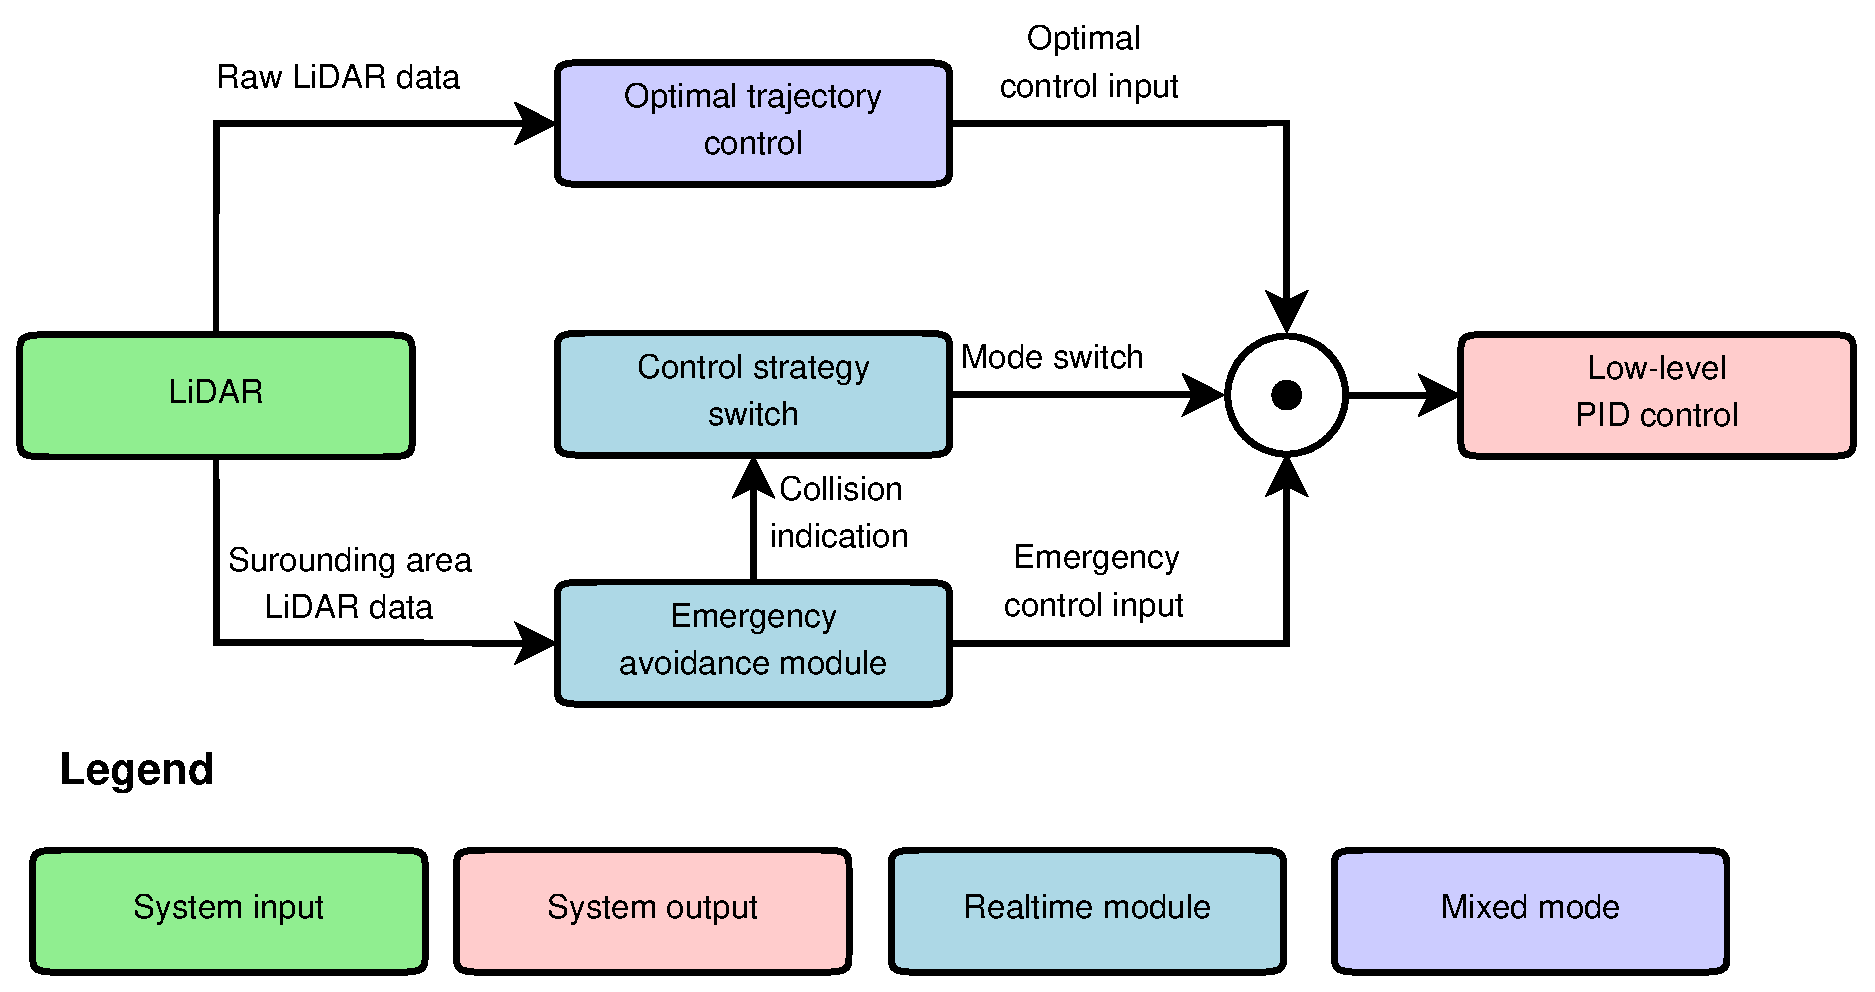
\includegraphics[width=\textwidth]{Pics/GlobalConcept.eps}
    \caption{Robust avoidance control concept scheme}
    \label{fig:GlobalConcept}
\end{figure}

\subsubsection{LiDAR}
LiDAR is planned to be used as main active data input. Low-density LiDAR \cite{url:kickstarter:lidar} can be used in UAV applications 
in standby mode or scan/sweep mode.
Low density LiDAR is ideal for feature extraction which is used mainly in Geographical Information Systems.

\begin{enumerate}[]
	\item \textbf{Role}
	    \begin{enumerate}[]
		    \item Data gathering of current vehicle surroundings
		\end{enumerate}
	\item \textbf{Output:}
	    \begin{enumerate}[1.]
		\item Point cloud of data
		\end{enumerate}
\end{enumerate}

\subsubsection{Control strategy switch}
TODO
\begin{enumerate}[]
	\item \textbf{Role}
	    \begin{enumerate}[]
		    \item TODO
		\end{enumerate}
	\item \textbf{Input:}
	    \begin{enumerate}[1.]
		\item TODO
		\end{enumerate}	
	\item \textbf{Output:}
	    \begin{enumerate}[1.]
		\item TODO
		\end{enumerate}
\end{enumerate}


\subsubsection{Emergency avoidance module}
TODO
\begin{enumerate}[]
	\item \textbf{Role}
	    \begin{enumerate}[]
		    \item TODO
		\end{enumerate}
	\item \textbf{Input:}
	    \begin{enumerate}[1.]
		\item TODO
		\end{enumerate}	
	\item \textbf{Output:}
	    \begin{enumerate}[1.]
		\item TODO
		\end{enumerate}
\end{enumerate}

\subsubsection{Optimal trajectory control}
TODO
\begin{enumerate}[]
	\item \textbf{Role}
	    \begin{enumerate}[]
		    \item TODO
		\end{enumerate}
	\item \textbf{Input:}
	    \begin{enumerate}[1.]
		\item TODO
		\end{enumerate}	
	\item \textbf{Output:}
	    \begin{enumerate}[1.]
		\item TODO
		\end{enumerate}
\end{enumerate}



\subsubsection{Low level PID control}
	Low level control of vehicle on desired trajectory
	\begin{enumerate}[]
	\item \textbf{Role:}
		\begin{enumerate}[]
		\item Low level control of vehicle motors ...
		\end{enumerate}
	\item \textbf{Input:}
		\begin{enumerate}[1.]
		\item Desired trajectory
		\end{enumerate}
	\item \textbf{Output:}
		\begin{enumerate}[2.]
		\item Control inputs 
		\end{enumerate}
	\end{enumerate}


